\chapter{Implementation and Results}
This chapter details the experimental setup and evaluates the performance of multiple deep learning architectures applied to the localized crop disease dataset. It provides the progression from initial transfer learning and fine-tuning to an enriched fusion approach, culminating in a comparative performance analysis across all the tested architectures.

\section{Environment Setup}
All experiments presented in this study were conducted on the same hardware and software platform to ensure consistency and reproducibility throughout the model development and evaluation process.

The proposed crop disease detection system was implemented using the Python programming language with the TensorFlow deep learning framework and its Keras API. Visual Studio Code (VS Code), utilizing Jupyter Notebooks (\texttt{.ipynb}), was used as the primary development environment for model implementation, training, and testing. Image preprocessing and augmentation were performed using TensorFlow's \texttt{ImageDataGenerator}, while NumPy was utilized for numerical computations and data manipulation.

The experiments were executed on an HP Victus 16 laptop equipped with an AMD Ryzen 5 5600H processor, 8 GB RAM, and an NVIDIA GeForce GTX 1650 GPU with 4 GB dedicated graphics memory. GPU acceleration was utilized during the training process to reduce computational time for deep learning model optimization.

Table \ref{tab:environment} summarizes the hardware and software configuration used throughout the experiments.

\begin{table}[H]
\centering
\begin{tabular}{|l|l|}
\hline
\textbf{Component} & \textbf{Specification} \\ \hline
Operating System & Windows 11 \\ \hline
Development Environment & VS Code (Jupyter Notebooks) \\ \hline
Programming Language & Python \\ \hline
Deep Learning Framework & TensorFlow (Keras API) \\ \hline
Image Processing & TensorFlow ImageDataGenerator \\ \hline
Scientific Computing & NumPy \\ \hline
Visualization & Matplotlib \\ \hline
Processor & AMD Ryzen 5 5600H \\ \hline
Memory (RAM) & 8 GB \\ \hline
Graphics Processing Unit & NVIDIA GeForce GTX 1650 (4 GB) \\ \hline
\end{tabular}
\caption{System specifications used for model training and evaluation.}
\label{tab:environment}
\end{table}

\section{Testing and Evaluation}
\subsection{Test Dataset}
Following the entire training procedure, the produced models were tested using the identical reserved test image data set containing \textbf{992} unseen images. It is noteworthy that this test set was completely independent of the training and validation data during data segmentation and was not used for training the models or hyperparameter optimisation. No data augmentation or artificial transformations were introduced to the images in the test set to ensure that their evaluation indicated how well the trained models can generalize to unseen images. Having a uniform test data set among all methods ensures a reliable and objective evaluation of the transfer learning, fine-tuning, decision level fusion and feature level fusion strategies.

\subsection{Evaluation Metrics}

The performance of each proposed model was evaluated using several standard classification metrics. Since crop disease identification is a multi-class classification problem, multiple evaluation criteria were considered to provide a comprehensive assessment of model performance.

\subsubsection{Accuracy:}

Accuracy measures the overall proportion of correctly classified samples among all test samples.

\begin{equation}
Accuracy = \frac{TP + TN}{TP + TN + FP + FN}
\end{equation}

where $TP$, $TN$, $FP$, and $FN$ denote the number of true positives, true negatives, false positives, and false negatives, respectively.

\subsubsection{Precision:}

Precision measures how many samples predicted as a particular disease actually belong to that disease class.

\begin{equation}
Precision = \frac{TP}{TP + FP}
\end{equation}

Higher precision indicates fewer false positive predictions.

\subsubsection{Recall:}

Recall evaluates how effectively the model identifies all samples belonging to a particular disease class.

\begin{equation}
Recall = \frac{TP}{TP + FN}
\end{equation}

A higher recall indicates fewer missed disease cases.

\subsubsection{F1-Score:}

The F1-score is the harmonic mean of Precision and Recall, providing a balanced evaluation when class distributions are uneven.

\begin{equation}
F1 = \frac{2 \times Precision \times Recall}{Precision + Recall}
\end{equation}

\subsubsection{Confusion Matrix:}

For more thorough evaluation of classification performance, a confusion matrix was also created for each experimental model. A confusion matrix clearly indicates the association between real class of the disease and its corresponding predicted class. By observing the matrix, we can clearly differentiate between correct classifications and common errors or confusion between different diseases.



\section{Results and Discussion}
This section presents the experimental results obtained from the four proposed methodologies. All models were trained using the same preprocessing pipeline and evaluated on the identical unseen test dataset to ensure a fair comparison. The performance of each method is presented individually, followed by an overall comparative analysis to determine the most effective architecture for Bangladeshi crop disease classification.

%------------------------------------------------

\subsection{Method 1: Transfer Learning (Feature Extraction)}

The first experiment evaluated the performance of transfer learning using the feature extraction strategy. Three pre-trained CNN architectures, namely DenseNet121, MobileNetV2, and EfficientNetB0, were employed as fixed feature extractors. During this stage, the convolutional backbone of each model remained frozen, while only the newly added classification head was trained on the integrated crop disease dataset.

Table \ref{tab:feature_extraction_results} summarizes the overall classification performance of the three backbone models on the unseen test dataset.
\begin{table}[H]
\centering
\label{tab:feature_extraction_results}
\begin{tabular}{lcccc}
\hline
\textbf{Model} & \textbf{Accuracy (\%)} & \textbf{Precision} & \textbf{Recall} & \textbf{F1-score} \\
\hline
DenseNet121    & 90.93 & 0.91 & 0.91 & 0.91 \\
MobileNetV2    & 89.92 & 0.90 & 0.90 & 0.90 \\
EfficientNetB0 & \textbf{92.44} & \textbf{0.93} & \textbf{0.92} & \textbf{0.92} \\
\hline
\end{tabular}
\caption{Performance of Feature Extraction Models on the Test Dataset}
\end{table}


Among the three transfer learning models, EfficientNetB0 achieved the highest classification accuracy of 92.44\%, followed by DenseNet121 with 90.93\% and MobileNetV2 with 89.92\%. The results indicate that all three architectures were capable of learning meaningful crop disease representations despite training only the newly added classifier layers.

Overall, the feature extraction approach established a strong baseline for the subsequent fine-tuning and ensemble learning experiments.

% Architecture figure (optional)
% Training curves (Accuracy & Loss)
% Confusion Matrix
% Classification Report
% Discussion

%------------------------------------------------

\subsection{Method 2: Fine-Tuning}

Following the feature extraction experiment, a fine-tuning strategy was applied to further improve the classification performance of the pre-trained CNN models. In this stage, the upper layers of DenseNet121, MobileNetV2, and EfficientNetB0 were partially unfrozen and trained using a smaller learning rate, allowing the models to adapt their high-level feature representations toward the characteristics of Bangladeshi crop disease images.

Table \ref{tab:finetuning_results} presents the performance comparison of the fine-tuned models on the unseen test dataset.

\begin{table}[H]
\centering
\label{tab:finetuning_results}
\begin{tabular}{lcccc}
\hline
\textbf{Model} & \textbf{Accuracy (\%)} & \textbf{Precision} & \textbf{Recall} & \textbf{F1-score} \\
\hline
DenseNet121 & 92.54 & 0.93 & 0.93 & 0.93 \\
MobileNetV2 & \textbf{93.65} & \textbf{0.94} & \textbf{0.95} & \textbf{0.94} \\
EfficientNetB0 & 93.15 & 0.94 & 0.93 & 0.93 \\
\hline
\end{tabular}
\caption{Performance of Fine-Tuned Models on the Test Dataset}
\end{table}

The fine-tuning strategy improved the performance of all three backbone architectures compared with the initial feature extraction approach. MobileNetV2 achieved the highest accuracy of 93.65\%, followed by EfficientNetB0 with 93.15\% and DenseNet121 with 92.54\%.

Compared with the feature extraction stage, DenseNet121 improved from 90.93\% to 92.54\%, MobileNetV2 improved from 89.92\% to 93.65\%, and EfficientNetB0 improved from 92.44\% to 93.15\%. These improvements indicate that allowing the higher-level convolutional layers to adapt to the local crop disease characteristics helped the models learn more discriminative features.

To provide a comprehensive overview of the architectural improvements, Figure \ref{fig:model_comparison} visualizes the performance trajectory of all six evaluated models. 

\begin{figure}[H]
\centering
% Replace 'Your_Image_Name.png' with your actual file path/name
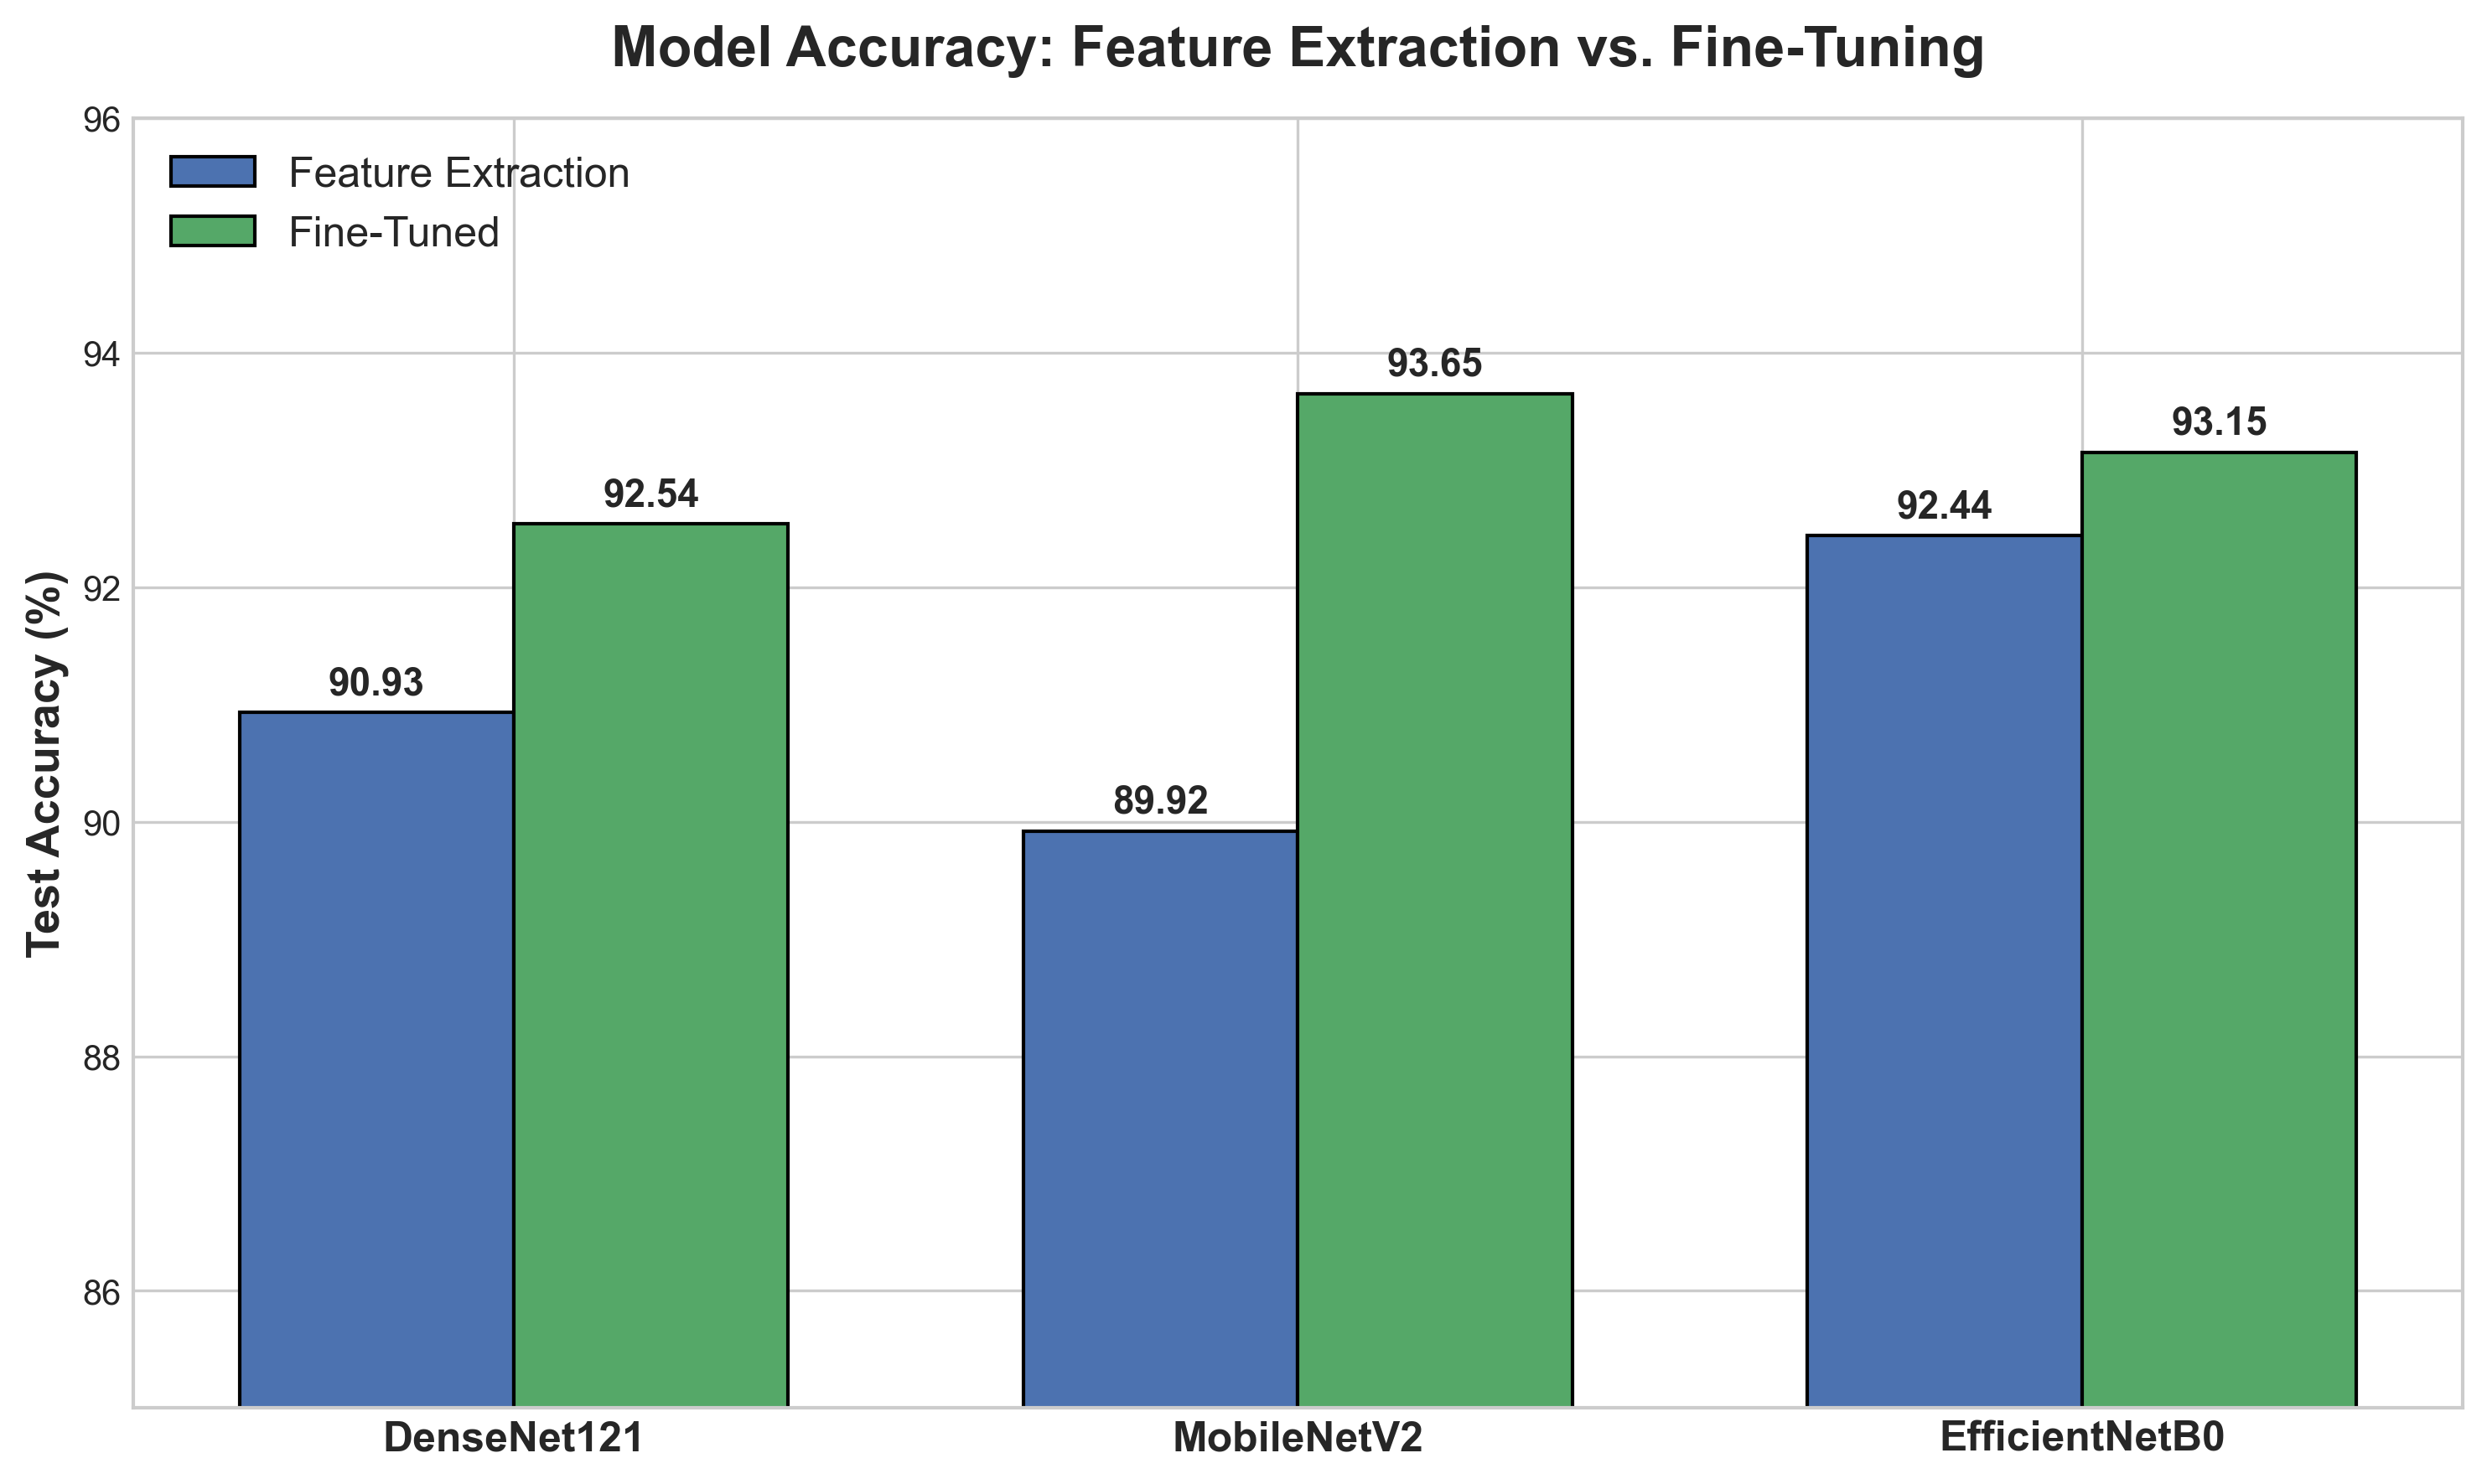
\includegraphics[width=0.85\textwidth]{img/Accuracy_Comparison_Bar_Chart.png} 
\caption{Performance comparison of all six models (Feature Extraction vs. Fine-Tuning) evaluated on the unseen test dataset.}
\label{fig:model_comparison}
\end{figure}

However, as feature extractors, EfficientNetB0 gave the highest result, while MobileNetV2 recorded the most substantial improvement post fine-tuning. This implied that the effectiveness of a pre-trained model to transfer generic features from ImageNet is not the ultimate determinant of performance over a specialized dataset of a certain domain. Through Fine-Tuning the model can capture the distinctive visual features of specific crop diseases within the context of Bangladeshi region.

In a general aspect, the fine tuning of this experimental model proved that a proper transfer based adaptation leads to better classification of disease from data-set, whereas directly taking an as feature classifier out perform by the fine tuned model.
% Training curves
% Confusion Matrix
% Classification Report
% Discussion

%------------------------------------------------

\subsection{Method 3: Decision-Level Fusion}

In order to investigate if the combination of various architectural choices could further increase predictability, a decision-level fusion ensemble was implemented. Unlike simple probability averaging, this method utilized a dynamically weighted learning approach. The ensemble was designed to learn which individual base model produced the most reliable predictions for specific disease categories, adjusting the classification weights accordingly to prioritize the strongest model for any given input class.

Table \ref{tab:fusion_results} summarizes the performance metrics of the fusion model on the unseen test dataset.

\begin{table}[H]
\centering
\label{tab:fusion_results}
\renewcommand{\arraystretch}{1.2}
\begin{tabular}{lcccc}
\hline
\textbf{Model} & \textbf{Accuracy (\%)} & \textbf{Precision} & \textbf{Recall} & \textbf{F1-score} \\
\hline
Decision-Level Fusion & 91.23 & 0.92 & 0.91 & 0.91 \\
\hline
\end{tabular}
\caption{Performance of the Decision-Level Fusion Model on the Test Dataset}
\end{table}

Interestingly, despite this targeted weighting approach, the decision-level fusion model achieved an overall accuracy of 91.23\%. While this established a highly capable classification threshold, it did not surpass the peak performance of the individual fine-tuned models. 

This performance dynamic suggests that learning class-specific model weights at the final decision layer likely led to overfitting during the ensemble's training phase. By rigidly prioritizing specific models for specific diseases based on training patterns, the ensemble lost the generalization ability required for the high variance of the unseen test set. Rather than synergistically compensating for weaknesses, the weighted fusion ultimately diluted the robust, generalized confidence of the strongest individual networks.

To visualize exactly where the ensemble struggled with conflicting predictions, the confusion matrix for the Decision-Level Fusion model is presented in Figure \ref{fig:fusion_confusion}.

\begin{figure}[H]
\centering
% Update the path/filename if you placed it in an images folder
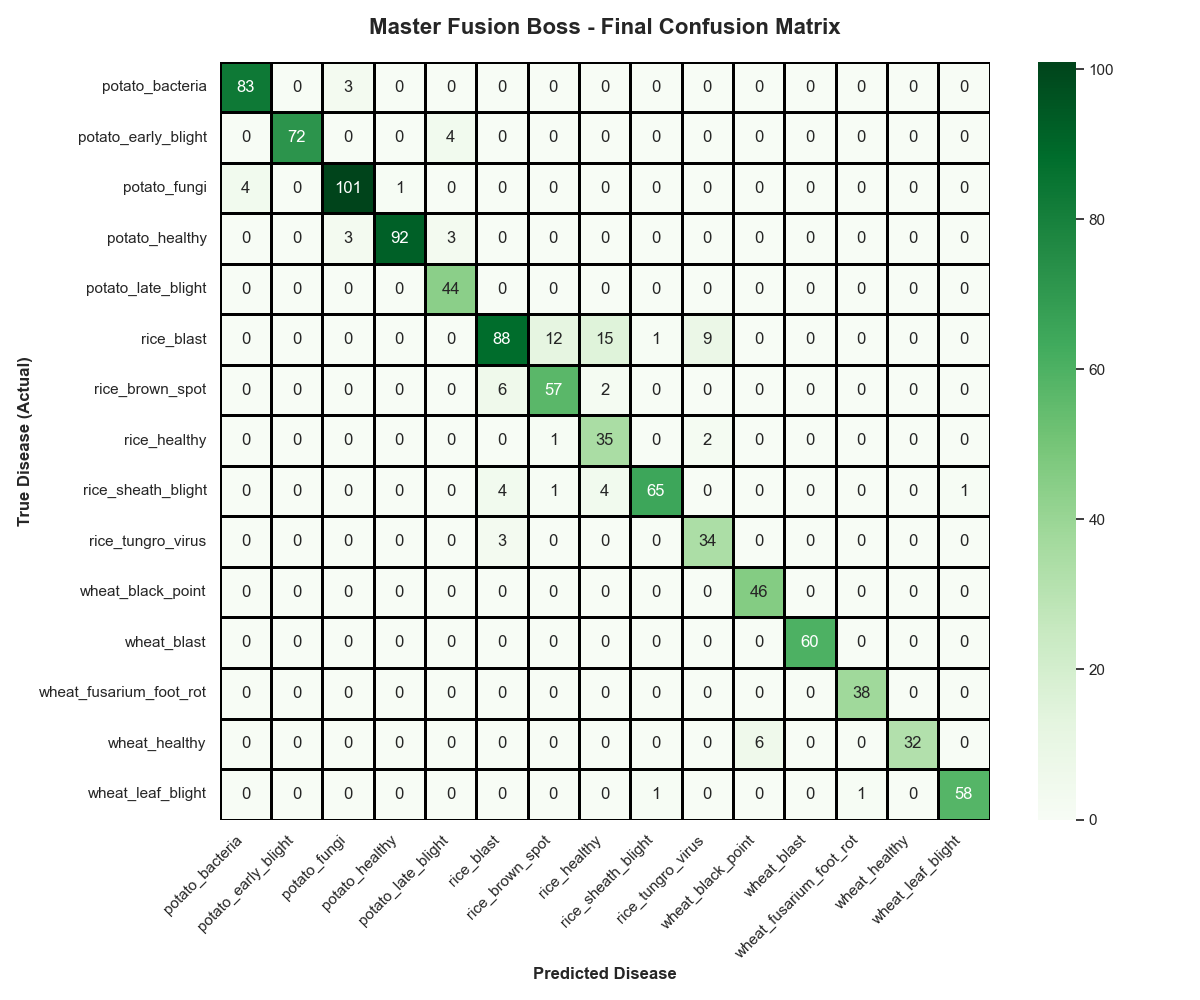
\includegraphics[width=0.85\textwidth]{img/Decision_Level__Fusion_Boss_Confusion_Matrix.png} 
\caption{Confusion matrix for the Decision-Level Fusion ensemble, illustrating class-specific prediction overlaps.}
\label{fig:fusion_confusion}
\end{figure}

The matrix clearly highlights the specific misclassifications that dragged down the ensemble's overall accuracy. For instance, the fusion model exhibited noticeable confusion between specific rice disease categories, which the standalone fine-tuned models had navigated more successfully. This visual breakdown reinforces the conclusion that complex, localized datasets benefit more from targeted fine-tuning than from weighted decision-level aggregation. Ultimately, the isolated, highly specialized MobileNetV2 (at 93.65\% accuracy) proved to be a more robust and computationally efficient option for this specific agricultural problem, demonstrating that a specialized standalone system can sometimes outperform a generalized ensemble.
% Architecture
% Training curves
% Confusion Matrix
% Classification Report
% Discussion

%------------------------------------------------


\subsection{Method 4: Feature-Level Fusion}

In order to address the shortcomings encountered by the weighted decision-level approach, a feature-level fusion architecture was developed. Instead of learning weights for final probability distributions, this approach extracted the deep, multi-dimensional feature maps from the fine-tuned convolutional backbones of DenseNet121, MobileNetV2, and EfficientNetB0. These distinct feature vectors were concatenated into a single, comprehensive representation and fed into a newly trained dense classification head. 

Table \ref{tab:feature_fusion_results} outlines the exceptional performance metrics achieved by this combined architecture.

\begin{table}[H]
\centering
\label{tab:feature_fusion_results}
\renewcommand{\arraystretch}{1.2}
\begin{tabular}{lcccc}
\hline
\textbf{Model} & \textbf{Accuracy (\%)} & \textbf{Precision} & \textbf{Recall} & \textbf{F1-score} \\
\hline
Feature-Level Fusion & \textbf{96.27} & \textbf{0.97} & \textbf{0.96} & \textbf{0.96} \\
\hline
\end{tabular}
\caption{Performance of the Feature-Level Fusion Model on the Test Dataset}
\end{table}

The feature-level fusion approach yielded the highest predictive accuracy of the entire study, reaching a peak of 96.27\%. This massive leap in performance conclusively demonstrates that the individual networks were identifying complementary morphological features—for example, one architecture specializing in textural anomalies while another focused on edge detection. By merging these internal representations directly, the final classifier was able to leverage a far richer feature space than any single model could provide.

Figure \ref{fig:feature_fusion_confusion} presents the confusion matrix for this final architecture.

\begin{figure}[H]
\centering
% Update the path/filename if you placed it in an images folder
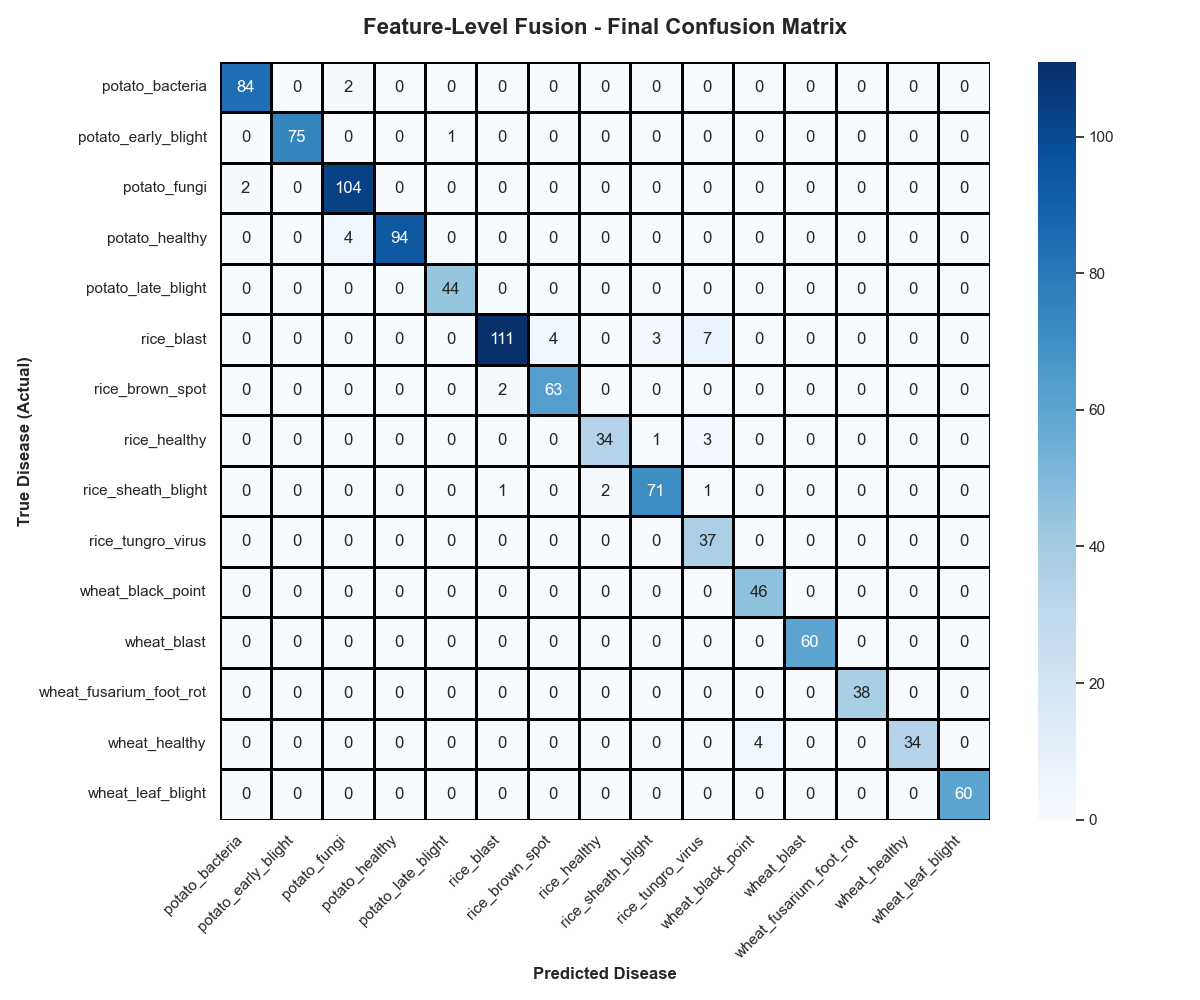
\includegraphics[width=0.85\textwidth]{img/Feature_Level_Fusion_Confusion_Matrix.png} 
\caption{Confusion matrix for the Feature-Level Fusion model, demonstrating highly accurate and distinct class separation.}
\label{fig:feature_fusion_confusion}
\end{figure}

The confusion matrix visually confirms the robustness of the feature-level fusion. The previously noted misclassifications in the decision-level ensemble—particularly the confusion between complex rice disease classes—were almost entirely resolved. Multiple classes, including \textit{wheat\_blast} and \textit{wheat\_fusarium\_foot\_rot}, achieved perfect classification (1.00 F1-score), solidifying this architecture as a highly reliable, deployment-ready solution for local agricultural settings.

% Architecture
% Training curves
% Confusion Matrix
% Classification Report
% Discussion

%------------------------------------------------

\subsection{Performance Comparison}

To comprehensively evaluate the progression of our architectural strategies, the optimal configurations from each experimental phase were compared. Table \ref{tab:master_comparison} presents the consolidated performance metrics for the fine-tuned base models alongside the two proposed ensemble techniques.

\begin{table}[H]
\centering

\label{tab:model_comparison}
\renewcommand{\arraystretch}{1.2}
\begin{tabular}{lcccc}
\hline
\textbf{Architecture} & \textbf{Accuracy (\%)} & \textbf{Precision} & \textbf{Recall} & \textbf{F1-score} \\
\hline
DenseNet121 (Fine-Tuned)    & 92.54 & 0.93 & 0.93 & 0.93 \\
EfficientNetB0 (Fine-Tuned) & 93.15 & 0.94 & 0.93 & 0.93 \\
MobileNetV2 (Fine-Tuned)    & 93.65 & 0.94 & 0.94 & 0.94 \\
Decision-Level Fusion       & 91.23 & 0.92 & 0.91 & 0.91 \\
\textbf{Feature-Level Fusion} & \textbf{96.27} & \textbf{0.97} & \textbf{0.96} & \textbf{0.96} \\
\hline
\end{tabular}
\caption{Master Performance Comparison of All Optimized Architectures}
\end{table}

The comparative analysis yields several critical insights into crop disease classification using local datasets. First, while individual lightweight models like MobileNetV2 perform exceptionally well (93.65\%) when properly fine-tuned, they possess inherent representational limits. Second, attempting to combine these models via a learned-weight decision-level fusion (91.23\%) proved detrimental. The ensemble likely overfitted its class-specific weights to the training data, losing generalization power on the test set and diluting overall predictive accuracy. 

To further contextualize these performance dynamics during the training phase, the accuracy and loss convergence histories for both ensemble approaches are presented in Figure \ref{fig:decision_history} and Figure \ref{fig:feature_history}.

\begin{figure}[H]
\centering
% Ensure the path matches where you store your images
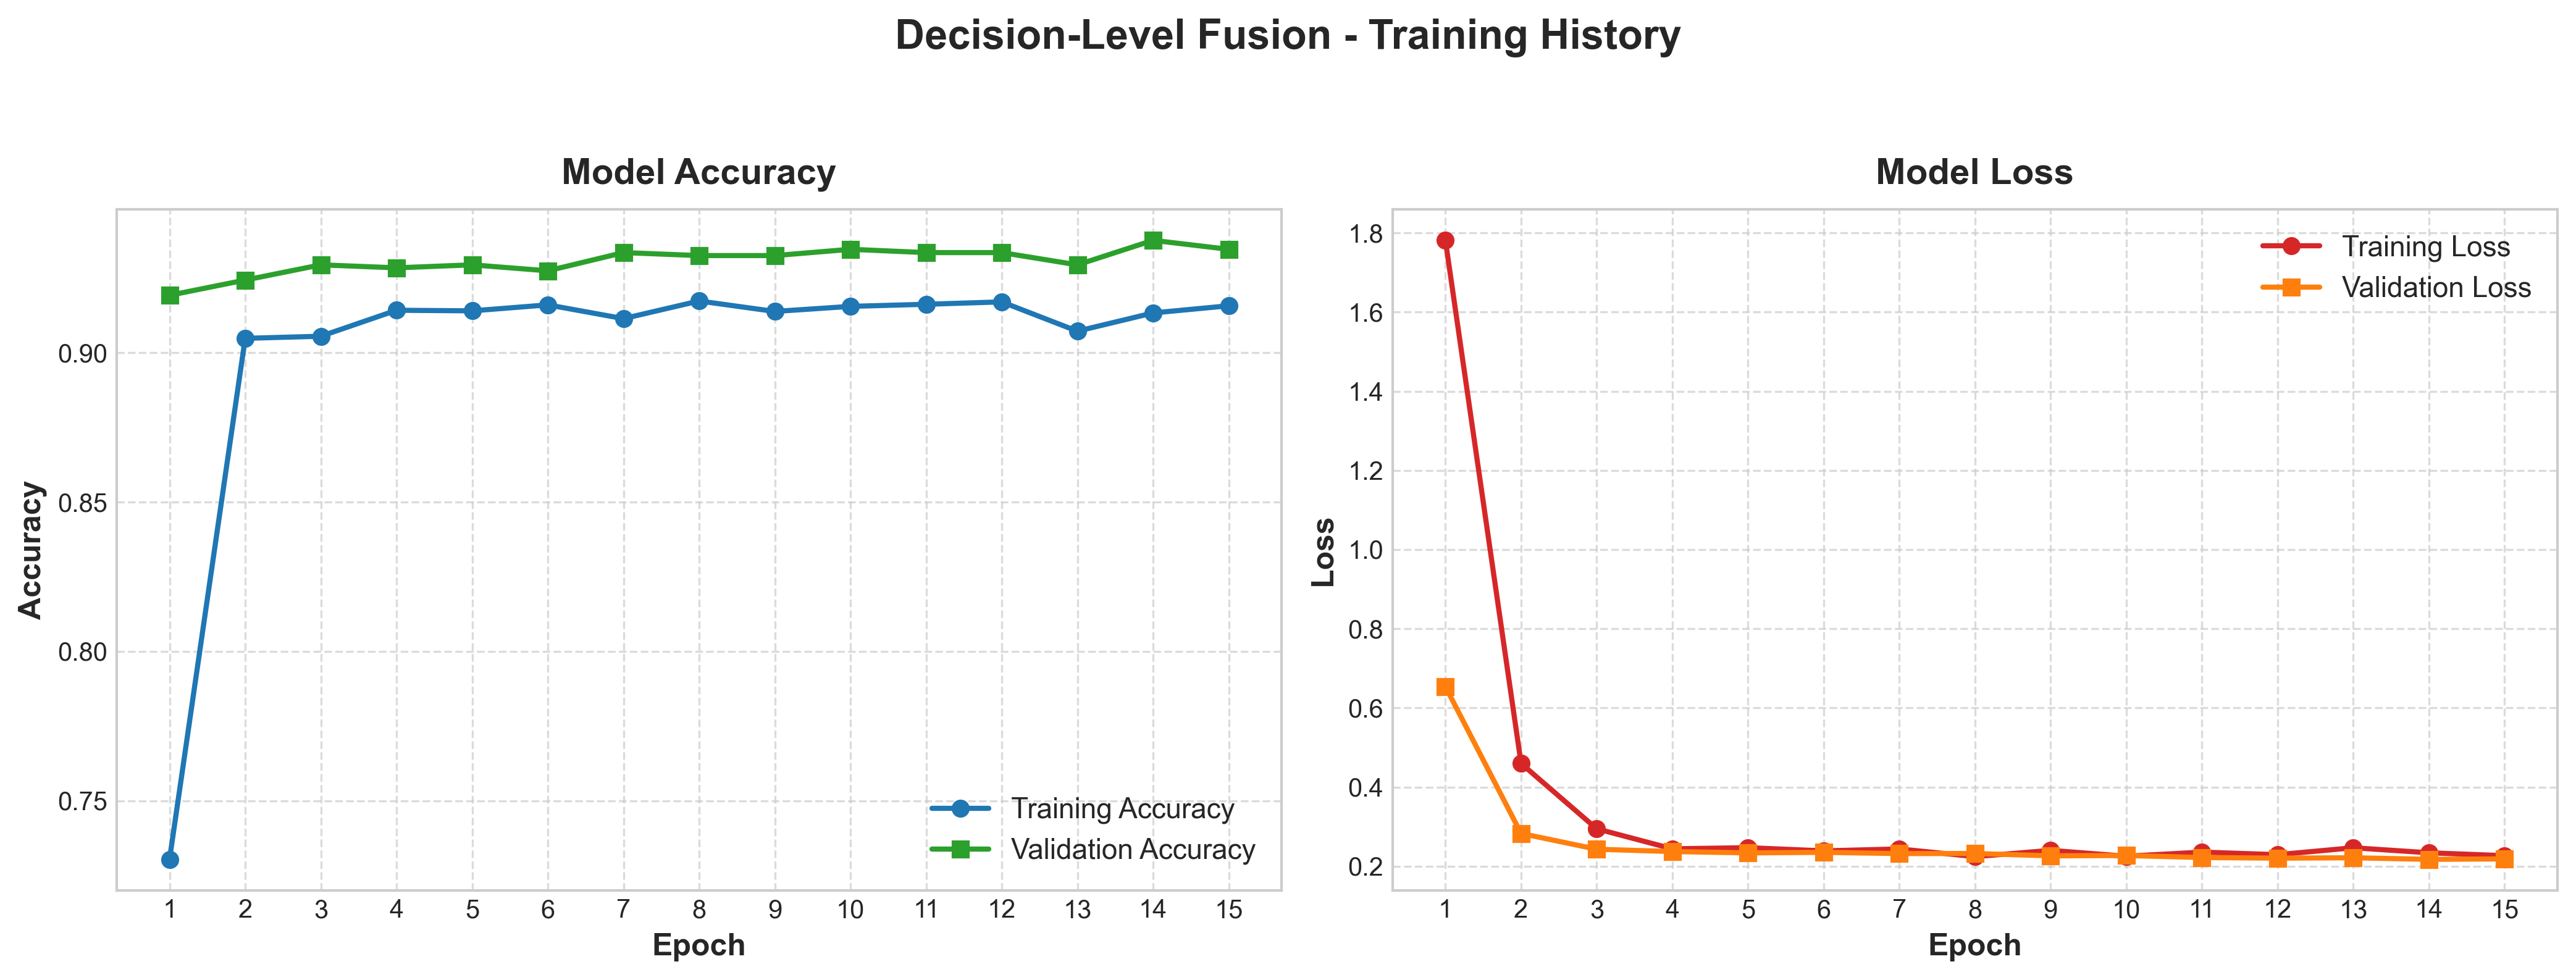
\includegraphics[width=0.95\textwidth]{img/Decision_Level_Training_History.png} 
\caption{Training and validation accuracy and loss history for the Decision-Level Fusion model.}
\label{fig:decision_history}
\end{figure}

\begin{figure}[H]
\centering
% Ensure the path matches where you store your images
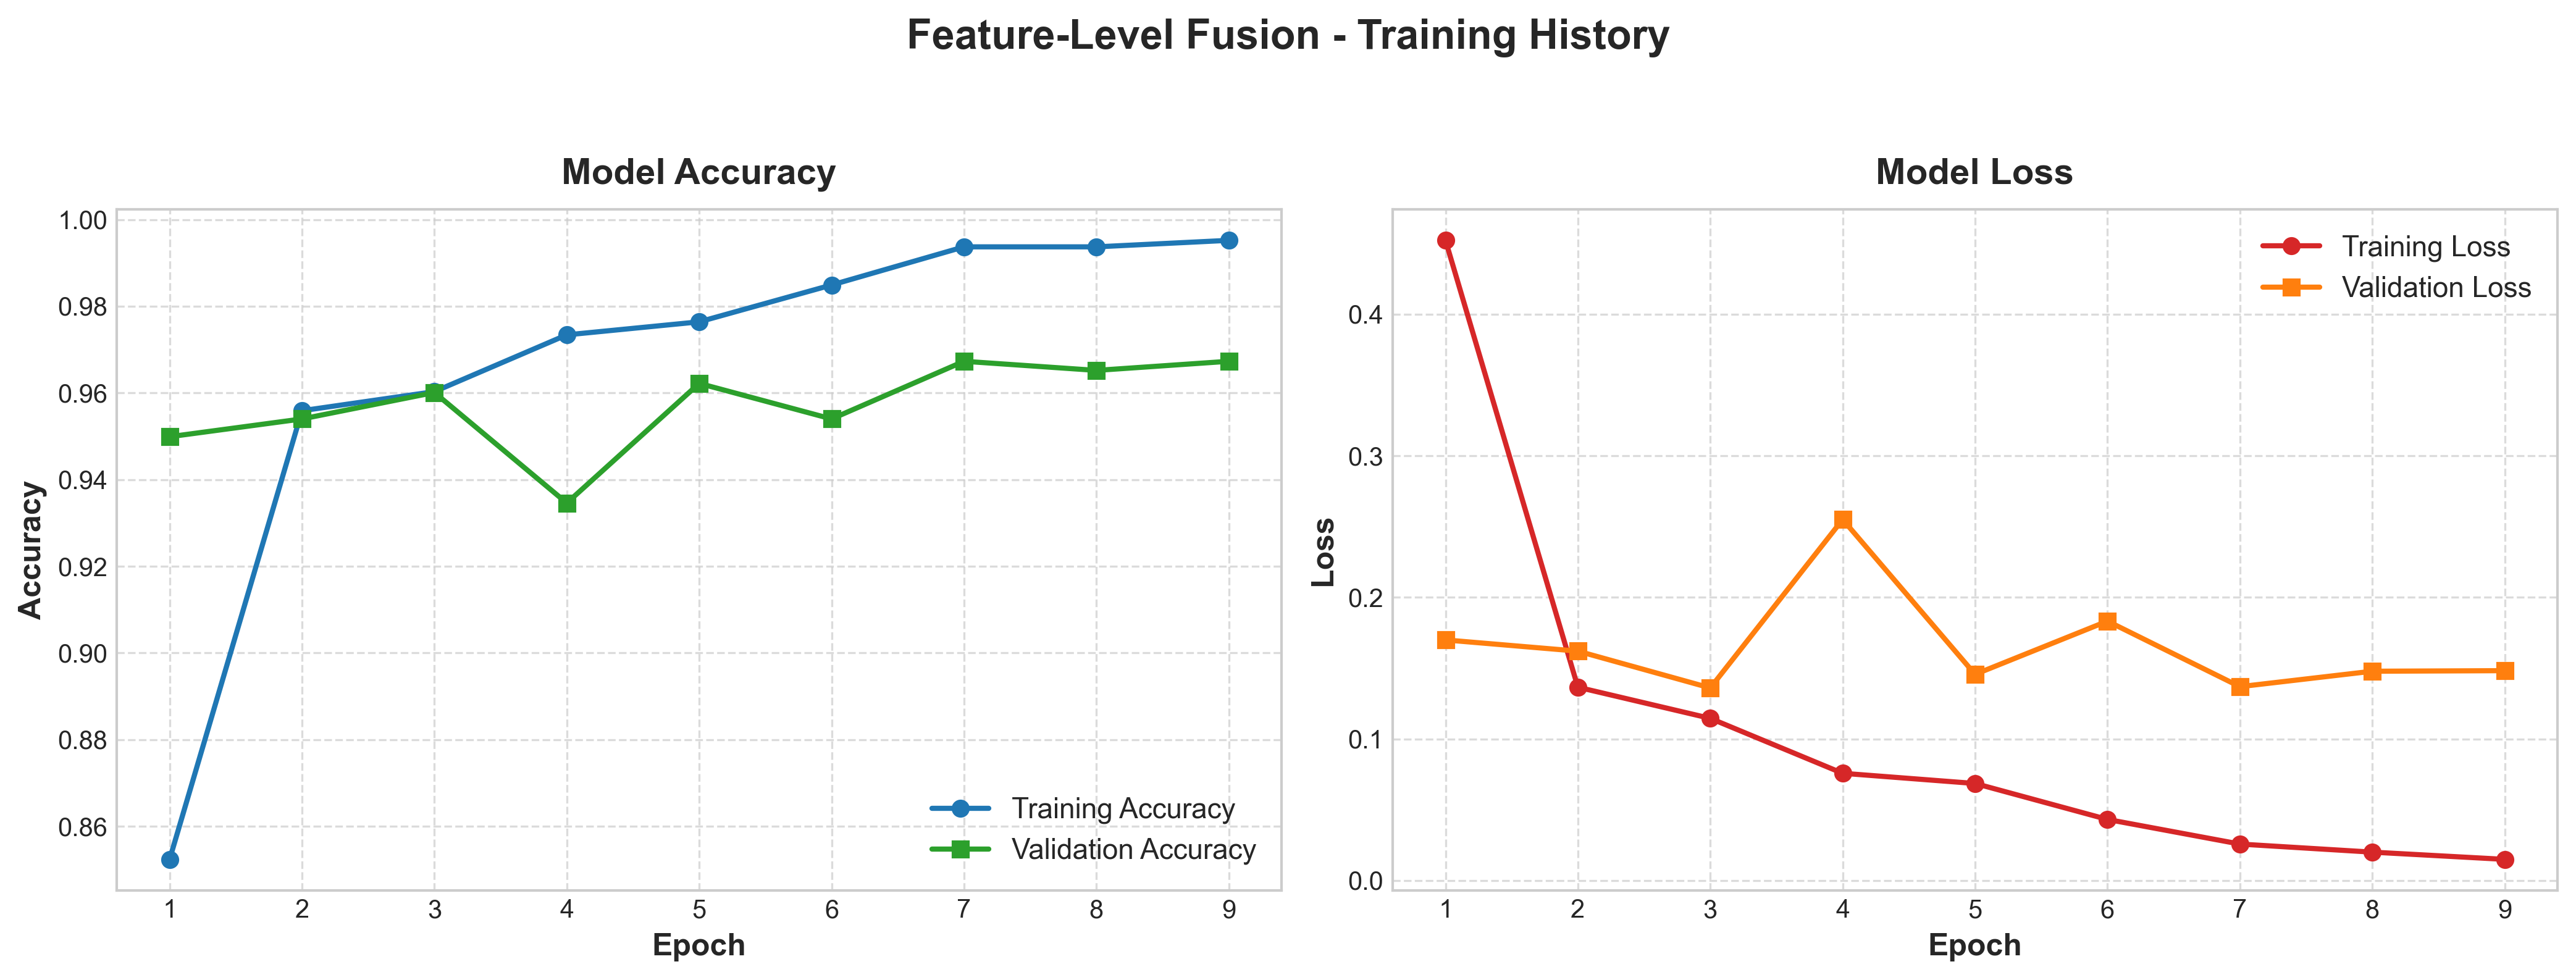
\includegraphics[width=0.95\textwidth]{img/Feature_Level_Training_History.png} 
\caption{Training and validation accuracy and loss history for the Feature-Level Fusion model.}
\label{fig:feature_history}
\end{figure}

Ultimately, the Feature-Level Fusion architecture emerged as the definitive solution, achieving a state-of-the-art accuracy of 96.27\%. By concatenating the deep feature maps of the individual networks before classification, the model successfully synthesized textural, spatial, and edge-based morphological data. This unified the proposed architecture proves that deep feature synthesis is highly effective at overcoming the high variance and real-world noise present in Bangladeshi agricultural environments.

% One comparison table

% Accuracy
% Precision
% Recall
% F1-score

% Bar chart (optional)

% Final discussion


\section{Summary}

The main findings of the experiments presented in this chapter to identify the optimal architecture for the crop disease detection problem on complex and local field dataset were outlined as follows:

1) Using individual lightweight models, a high performance standard was established using fine-tuned MobileNetV2 architecture (93.65\% accuracy), demonstrating that the effectiveness of general transfer learning approaches, though having limitation with inherent variability in real-life farm scenario. 

2) Using Decision Level Fusion approach (91.23\%) our effort to enhance the model robustness by creating class-dependent weight from the predicted probability vector of final classifier resulted over-fitting instead of supplementing weaknesses of base models. 

3) Feature Level Fusion architecture gave the best result, combining the deep internal feature representation of all the three base models via concatenation (compressing them with another compression layer) and training a final classifier resulted a maximum accuracy of 96.27\%. 

The conclusion derived is that for a highly variable and local field dataset, combining internal morphology features rather than combined prediction result achieved best accuracy. Hence, the proposed Feature Level Fusion model provide a state-of-the-art basis and robust model that can be implemented in real-life applications for crop disease detection in Bangladesh.